% TeleCon control protocol — technical reference + Bluetooth examples.
% Build: pdflatex -output-directory=../build telecon_control_protocol.tex
\documentclass[12pt,a4paper]{article}

\usepackage[margin=2.4cm]{geometry}
\usepackage[T1]{fontenc}
\usepackage[utf8]{inputenc}
\usepackage{lmodern}
\usepackage{booktabs}
\usepackage{hyperref}
\usepackage{xcolor}
\usepackage{colortbl}
\usepackage{array}
\usepackage{enumitem}
\usepackage{needspace}
\usepackage{etoolbox}
\usepackage{tikz}
\usepackage{listings}
\usepackage{verbatim}

\usetikzlibrary{arrows.meta,calc,fit}
\preto\section{\Needspace{10\baselineskip}}

\hypersetup{
  colorlinks=true,
  linkcolor=black,
  urlcolor=blue,
  pdftitle={TeleCon Control Protocol},
  pdfauthor={TeleCon}
}

% Arduino IDE 2 syntax colors (readable on the light listing background).
\definecolor{ArduinoKeyword}{HTML}{00979C}
\definecolor{ArduinoFunc}{HTML}{D35400}
\definecolor{ArduinoString}{HTML}{D35400}
\definecolor{ArduinoComment}{HTML}{5D6D6E}
\definecolor{ArduinoPreproc}{HTML}{9B59B6}

% Semantic colors for byte-layout / field tables.
\definecolor{TblHead}{HTML}{0F6F73}
\definecolor{TblSync}{HTML}{E8DAEF}
\definecolor{TblChan}{HTML}{D5F5E3}
\definecolor{TblKnob}{HTML}{D6EAF8}
\definecolor{TblSw}{HTML}{FCF3CF}
\definecolor{TblSum}{HTML}{FAD7A0}
\definecolor{TblEnd}{HTML}{E5E7E9}
\definecolor{TblTelem}{HTML}{D4E6F1}
\definecolor{TblId}{HTML}{F5CBA7}
\definecolor{TblLen}{HTML}{FDEBD0}

\newcommand{\thc}[1]{\textcolor{white}{\bfseries #1}}
\newcommand{\chip}[2]{\colorbox{#1}{\strut\,\scriptsize #2\,}}
\newcommand{\mapcell}[3]{%
  \cellcolor{#1}%
  \begin{tabular}{@{}c@{}}
    \strut\textbf{\texttt{#2}}\\[-1pt]
    \scriptsize #3
  \end{tabular}%
}

\definecolor{WireApp}{HTML}{0F6F73}
\definecolor{WireType}{HTML}{9B59B6}
\definecolor{WireKey}{HTML}{1A5276}
\definecolor{WireVal}{HTML}{D35400}
\definecolor{WireSep}{HTML}{7F8C8D}
\definecolor{WireBg}{HTML}{F4FBFC}

\newcommand{\wapp}[1]{\textcolor{WireApp}{\textbf{\texttt{#1}}}}
\newcommand{\wtyp}[1]{\textcolor{WireType}{\textbf{\texttt{#1}}}}
\newcommand{\wkey}[1]{\textcolor{WireKey}{\texttt{#1}}}
\newcommand{\wval}[1]{\textcolor{WireVal}{\texttt{#1}}}
\newcommand{\wsep}{\textcolor{WireSep}{\texttt{,}}\hspace{0pt}}
\newcommand{\wcol}{\textcolor{WireSep}{\texttt{:}}}

\tikzset{
  telecon actor/.style={
    rounded corners=4pt,
    minimum width=2.7cm,
    minimum height=1.05cm,
    font=\sffamily\bfseries,
    text=white,
    inner sep=4pt
  },
  telecon step/.style={
    circle,
    inner sep=1pt,
    minimum size=0.52cm,
    font=\sffamily\bfseries\scriptsize,
    text=white
  },
  telecon pill/.style={
    rounded corners=2.5pt,
    inner sep=3.2pt,
    font=\ttfamily\scriptsize,
    align=center
  },
  telecon arr/.style={-{Latex[length=2.1mm]}, line width=0.9pt}
}

\newcommand{\wireframe}[1]{%
  \par\addvspace{0.55em}%
  \noindent
  {\setlength{\fboxrule}{1.1pt}%
   \setlength{\fboxsep}{8pt}%
   \fcolorbox{WireApp}{WireBg}{%
     \begin{minipage}{\dimexpr\linewidth-16pt-2.2pt\relax}
     \raggedright #1
     \end{minipage}}}%
  \par\addvspace{0.35em}%
}

\lstdefinestyle{Arduino}{
  language=C++,
  basicstyle=\ttfamily\normalsize\color{black},
  identifierstyle=\ttfamily\normalsize\color{black},
  keywordstyle=\ttfamily\normalsize\color{ArduinoKeyword}\bfseries,
  keywordstyle=[2]\ttfamily\normalsize\color{ArduinoFunc},
  keywordstyle=[3]\ttfamily\normalsize\color{ArduinoKeyword},
  commentstyle=\ttfamily\normalsize\color{ArduinoComment}\itshape,
  stringstyle=\ttfamily\normalsize\color{ArduinoString},
  directivestyle=\ttfamily\normalsize\color{ArduinoPreproc}\bfseries,
  morekeywords={
    String,boolean,byte,word,nullptr,size_t,
    uint8_t,uint16_t,uint32_t,uint64_t,
    int8_t,int16_t,int32_t,int64_t
  },
  morekeywords=[2]{
    setup,loop,print,println,begin,available,read,trim,
    indexOf,substring,length,startsWith,toInt,c_str,hasClient,
    strtol,valueOf,sendLine,applyOutputs,handleConnect,handleCtrl,
    handleLine,sendTelemetry,sendPlot,sendData,toPlotByte,
    millis,constrain,map,abs,snprintf,analogRead
  },
    morekeywords=[3]{SERIAL_8N1,SERIAL_BAUD,HIGH,LOW,INPUT,OUTPUT,INPUT_PULLUP}
}

\lstset{
  style=Arduino,
  breaklines=true,
  columns=fullflexible,
  frame=single,
  xleftmargin=0.3em,
  xrightmargin=0.3em,
  framesep=3pt,
  backgroundcolor=\color{gray!8},
  showstringspaces=false,
  keepspaces=true
}

\title{TeleCon Control Protocol\\[0.4em]
\large Byte-stream contract with the Android application}
\author{Firmware reference --- any MCU that implements this contract}
\date{Version 1.2 \quad 2026}

\begin{document}
\maketitle

\begin{abstract}
This document specifies how firmware must exchange bytes with TeleCon4ESP32
over Classic Bluetooth SPP, BLE Nordic UART, or TCP.
The application is transport-agnostic: it does not require an Espressif SoC,
a particular GAP name, or vendor AT commands.
Official Arduino sketches are reference implementations of this contract,
not part of the wire definition.

Control Panel and RC Vehicle Pro share the application prefix \texttt{RC}.
HTTP camera streaming (\texttt{/stream}, \texttt{/capture}) is a separate
session and is out of scope.
\end{abstract}

\section{Architecture}
\label{sec:arch}

The phone is always the client. After the underlying link is established,
it runs an application-layer session. Three layers must be implemented
on the device:

\begin{enumerate}[leftmargin=1.6cm]
  \item \textbf{Transport} --- a reliable-enough bidirectional octet stream
        (Section~\ref{sec:pipes}).
  \item \textbf{Session handshake} --- one text \texttt{CONNECT} line and an
        \texttt{ACK}/\texttt{NAK} reply (Section~\ref{sec:handshake}).
        Timeout on the phone is $2.5$\,s. Until ACK, UI control is not a
        live TeleCon session even if the OS reports the socket as connected.
  \item \textbf{Payload} --- Simple text lines (Section~\ref{sec:simple}) or
        Binary frames (Section~\ref{sec:binary}), selected by the user in
        application settings and echoed in \texttt{CONNECT}'s \texttt{proto}
        field.
\end{enumerate}

\Needspace{13.2cm}
\begin{center}
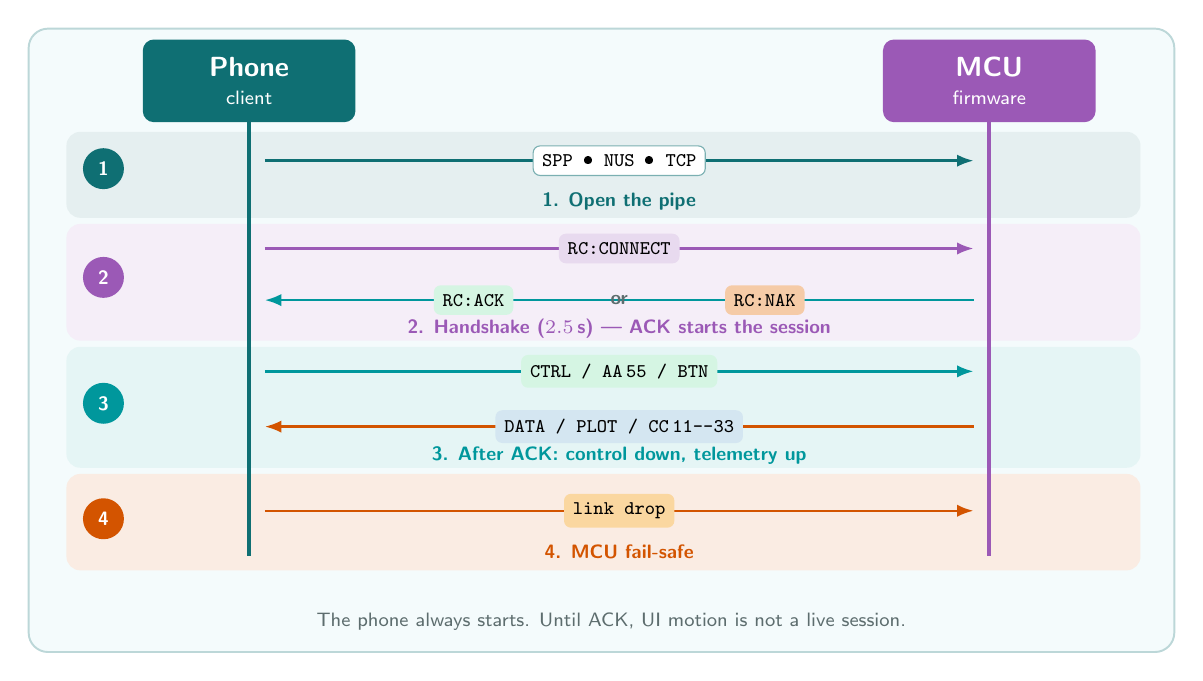
\begin{tikzpicture}[x=1cm, y=0.78cm]
  \fill[rounded corners=7pt, WireBg] (-0.4,-1.45) rectangle (14.15,8.7);
  \draw[rounded corners=7pt, TblHead!28, line width=0.7pt]
    (-0.4,-1.45) rectangle (14.15,8.7);

  \fill[TblHead!11, rounded corners=5pt] (0.08,5.62) rectangle (13.72,7.02);
  \fill[ArduinoPreproc!10, rounded corners=5pt] (0.08,3.62) rectangle (13.72,5.52);
  \fill[ArduinoKeyword!10, rounded corners=5pt] (0.08,1.55) rectangle (13.72,3.52);
  \fill[ArduinoFunc!11, rounded corners=5pt] (0.08,-0.12) rectangle (13.72,1.45);

  \node[telecon actor, fill=TblHead, align=center] at (2.4,7.85)
    {Phone\\[-1.6pt]{\normalfont\sffamily\scriptsize client}};
  \node[telecon actor, fill=ArduinoPreproc, align=center] at (11.8,7.85)
    {MCU\\[-1.6pt]{\normalfont\sffamily\scriptsize firmware}};
  \draw[TblHead, line width=1.4pt] (2.4,7.22) -- (2.4,0.12);
  \draw[ArduinoPreproc, line width=1.4pt] (11.8,7.22) -- (11.8,0.12);

  \node[telecon step, fill=TblHead] at (0.55,6.42) {1};
  \draw[telecon arr, TblHead] (2.6,6.55) -- (11.6,6.55);
  \node[telecon pill, fill=white, draw=TblHead!55] at (7.1,6.55)
    {SPP \textbullet\ NUS \textbullet\ TCP};
  \node[font=\sffamily\scriptsize\bfseries, text=TblHead] at (7.1,5.88)
    {1. Open the pipe};

  \node[telecon step, fill=ArduinoPreproc] at (0.55,4.65) {2};
  \draw[telecon arr, ArduinoPreproc] (2.6,5.12) -- (11.6,5.12);
  \node[telecon pill, fill=TblSync] at (7.1,5.12) {RC:CONNECT};
  \draw[telecon arr, ArduinoKeyword] (11.6,4.28) -- (2.6,4.28);
  \node[telecon pill, fill=TblChan] at (5.25,4.28) {RC:ACK};
  \node[font=\sffamily\scriptsize\bfseries, text=ArduinoComment] at (7.1,4.28)
    {or};
  \node[telecon pill, fill=TblId] at (8.95,4.28) {RC:NAK};
  \node[font=\sffamily\scriptsize\bfseries, text=ArduinoPreproc] at (7.1,3.82)
    {2. Handshake ($2.5$\,s) --- ACK starts the session};

  \node[telecon step, fill=ArduinoKeyword] at (0.55,2.6) {3};
  \draw[telecon arr, ArduinoKeyword] (2.6,3.12) -- (11.6,3.12);
  \node[telecon pill, fill=TblChan] at (7.1,3.12) {CTRL / AA\,55 / BTN};
  \draw[telecon arr, ArduinoFunc] (11.6,2.22) -- (2.6,2.22);
  \node[telecon pill, fill=TblTelem] at (7.1,2.22) {DATA / PLOT / CC\,11--33};
  \node[font=\sffamily\scriptsize\bfseries, text=ArduinoKeyword] at (7.1,1.75)
    {3. After ACK: control down, telemetry up};

  \node[telecon step, fill=ArduinoFunc] at (0.55,0.72) {4};
  \draw[telecon arr, ArduinoFunc] (2.6,0.85) -- (11.6,0.85);
  \node[telecon pill, fill=TblSum] at (7.1,0.85) {link drop};
  \node[font=\sffamily\scriptsize\bfseries, text=ArduinoFunc] at (7.1,0.18)
    {4. MCU fail-safe};

  \node[font=\sffamily\scriptsize, text=ArduinoComment] at (7.0,-0.95)
    {The phone always starts. Until ACK, UI motion is not a live session.};
\end{tikzpicture}

\vspace{0.3em}
{\sffamily\scriptsize
\chip{TblHead!18}{\textcolor{TblHead}{\textbf{1} pipe}}
\chip{TblSync}{\textbf{2} CONNECT}
\chip{TblChan}{ACK / CTRL}
\chip{TblId}{NAK}
\chip{TblTelem}{DATA / PLOT}
\chip{TblSum}{\textbf{4} drop}}

\vspace{0.15em}
{\sffamily\scriptsize\itshape
Phone--MCU flow. Green = accept, orange = reject, teal = control, blue = telemetry.}
\end{center}

The Bluetooth advertised name is GAP/SDP presentation only
(for example \texttt{ESP32-TC-RC-BT-Simple} on official firmware).
The handshake parser never matches the substring \texttt{ESP32}.
Connect uses the remote \textbf{address} plus SPP UUID or NUS attributes.

\subsection{Mode coupling}

The firmware's transport and payload must match the stored
\texttt{BluetoothConnectionMode}:

\begin{center}
\renewcommand{\arraystretch}{1.25}
\begin{tabular}{>{\raggedright\arraybackslash}p{3.5cm}
                >{\centering\arraybackslash}p{2.3cm}
                >{\centering\arraybackslash}p{1.8cm}
                >{\raggedright\arraybackslash}p{3.8cm}}
\rowcolor{TblHead}
\thc{Application mode} & \thc{Transport} & \thc{proto} & \thc{Payload after ACK} \\
\rowcolor{TblChan}
Classic Simple & SPP & \texttt{simple} & Section~\ref{sec:simple} \\
\rowcolor{TblTelem}
Classic Binary & SPP & \texttt{binary} & Section~\ref{sec:binary} \\
\rowcolor{TblTelem}
BLE Binary & NUS & \texttt{binary} & Section~\ref{sec:binary} \\
\rowcolor{TblTelem}
Wi-Fi SoftAP Binary & TCP :3333 & \texttt{binary} & Section~\ref{sec:binary} \\
\rowcolor{TblChan}
CAM starter (Role~B) & TCP :3333 & \texttt{simple} & Section~\ref{sec:simple} \\
\rowcolor{TblTelem}
CAM SoftAP Binary & TCP :3333 & \texttt{binary} & Section~\ref{sec:binary} \\
\rowcolor{TblId}
Legacy CAM SoftAP & TCP :3333 & \texttt{wifi} & Simple text \\
\end{tabular}

\vspace{0.4em}
\chip{TblChan}{Simple}
\chip{TblTelem}{Binary}
\chip{TblId}{Legacy Simple}
\end{center}

BLE is Binary-only in the current application.
A custom GATT serial profile (typical HM-10 UUIDs) will fail service
discovery: the client looks up Nordic UART only.

Mismatch should be signalled with \texttt{NAK} (\texttt{expected} = device
capability, \texttt{actual} = value from \texttt{CONNECT}).
Silent ignore produces \texttt{HandshakeFailure.Timeout} on the phone.

\section{Transports}
\label{sec:pipes}

\subsection{Classic SPP (RFCOMM)}

Serial Port Profile, UUID
\texttt{00001101-0000-1000-8000-00805F9B34FB}.

The Android client attempts, in order: secure
\texttt{createRfcommSocketToServiceRecord}, insecure
\texttt{createInsecureRfcommSocketToServiceRecord}, then a reflective
RFCOMM socket on channel~1.
The third attempt exists because some stacks (including ESP32
\texttt{BluetoothSerial} while a SoftAP \texttt{WifiNetworkSpecifier} is
held) fail SDP UUID lookup.

HC-05 / HC-06 expose this UUID as a transparent UART bridge.
The MCU only implements the byte protocol on that UART; baud is a module
setting (commonly 9600 or 115200), not negotiated by the phone.

\subsection{BLE Nordic UART Service}

\begin{center}
\renewcommand{\arraystretch}{1.25}
\begin{tabular}{>{\raggedright\arraybackslash}p{4.4cm}
                >{\raggedright\arraybackslash}p{6.2cm}
                >{\centering\arraybackslash}p{2.7cm}}
\rowcolor{TblHead}
\thc{Attribute on the peripheral} & \thc{UUID} & \thc{Role} \\
\rowcolor{TblSync}
Primary service &
  {\small\ttfamily 6E400001-\allowbreak B5A3-F393-\allowbreak E0A9-\allowbreak E50E24DCCA9E} &
  Service \\
\rowcolor{TblChan}
RX (Write / Write Without Response) &
  {\small\ttfamily 6E400002-\ldots CCA9E} &
  Phone $\rightarrow$ device \\
\rowcolor{TblTelem}
TX (Notify) &
  {\small\ttfamily 6E400003-\ldots CCA9E} &
  Device $\rightarrow$ phone \\
\rowcolor{TblLen}
CCCD on TX &
  {\small\ttfamily 00002902-\allowbreak 0000-1000-\allowbreak 8000-\allowbreak 00805F9B34FB} &
  Enable notify \\
\end{tabular}

\vspace{0.4em}
\chip{TblSync}{Service}
\chip{TblChan}{Phone writes}
\chip{TblTelem}{Device notifies}
\chip{TblLen}{Client config}
\end{center}

The client writes protocol octets to RX and reassembles TX notifications
into the same stream used for SPP.
Each notify/write must be $\le$ MTU$-3$.
Default ATT MTU 23 implies 20-byte chunks; request a larger MTU if you
send Binary frames in one shot.
Handshake text is still newline-delimited ASCII on this stream.

\subsection{TCP}

Same session and payload as Classic, on a single TCP connection.
Official SoftAP firmware binds \texttt{192.168.4.1:3333}.
Host/port are not part of the application protocol; they are deployment
parameters.
Do not invent a second handshake for TCP.

\section{Text encoding}

Handshake and Simple messages. Colour marks each token's job:

\begin{center}
\setlength{\tabcolsep}{4pt}
\renewcommand{\arraystretch}{1.15}
\begin{tabular}{|*{6}{>{\centering\arraybackslash}p{1.85cm}|}}
\hline
\mapcell{TblChan}{APP}{app} &
\mapcell{TblSync}{TYPE}{type} &
\mapcell{TblKnob}{key1}{key} &
\mapcell{TblId}{value1}{value} &
\mapcell{TblKnob}{key2}{key} &
\mapcell{TblId}{value2}{value} \\
\hline
\end{tabular}
\end{center}

\wireframe{%
\wapp{APP}\wcol\wtyp{TYPE}\wsep
\wkey{key1}\wsep\wval{value1}\wsep
\wkey{key2}\wsep\wval{value2}\wsep\texttt{...}%
}

\begin{center}
\vspace{-0.15em}
\chip{TblChan}{App}
\chip{TblSync}{Type}
\chip{TblKnob}{Key}
\chip{TblId}{Value}
\end{center}

Terminated by \texttt{LF} (\texttt{0x0A}). A preceding \texttt{CR} is
stripped.
\texttt{APP} for this product is \texttt{RC}.
Keys are case-sensitive as sent by the phone (\texttt{proto}, \texttt{lx},
\ldots).

Boolean values: \texttt{1}/\texttt{0}, \texttt{true}/\texttt{false},
\texttt{on}/\texttt{off}, or any non-zero integer.

The inbound assembler treats a leading \texttt{0xCC} as the start of a
Binary telemetry frame and printable ASCII as text.
After ACK in Binary mode, \texttt{0xAA}/\texttt{0xBB} are phone-to-device
control frames (they do not go through the text line parser on the device
unless you implement that yourself).

\section{Session handshake}
\label{sec:handshake}

Required on every new SPP, NUS, or TCP connection.
Not used for HTTP camera.

\subsection{Client $\rightarrow$ device}

\wireframe{%
\wapp{RC}\wcol\wtyp{CONNECT}\wsep\wkey{proto}\wsep\wval{simple}\\[0.25em]
\wapp{RC}\wcol\wtyp{CONNECT}\wsep\wkey{proto}\wsep\wval{binary}\\[0.25em]
\wapp{RC}\wcol\wtyp{CONNECT}\wsep\wkey{proto}\wsep\wval{wifi}%
}

\begin{center}
\vspace{-0.15em}
\chip{TblChan}{App}
\chip{TblSync}{Type}
\chip{TblKnob}{Key}
\chip{TblId}{Value}
\end{center}

\texttt{wifi} is retained for legacy one-board CAM SoftAP.
New Simple firmware should accept both \texttt{simple} and \texttt{wifi}
and emit the same ACK.

The phone waits $2500$\,ms for a line with the same app prefix \texttt{RC}
and type \texttt{ACK} or \texttt{NAK}.

\subsection{Device $\rightarrow$ client}

\wireframe{%
\wapp{RC}\wcol\wtyp{ACK}\wsep\wkey{app}\wsep\wval{RC}%
}

Additional ACK keys are ignored for session establishment.

\wireframe{%
\wapp{RC}\wcol\wtyp{NAK}\wsep
\wkey{reason}\wsep\wval{proto\_mismatch}\wsep
\wkey{expected}\wsep\wval{simple}\wsep
\wkey{actual}\wsep\wval{binary}\\[0.25em]
\wapp{RC}\wcol\wtyp{NAK}\wsep
\wkey{reason}\wsep\wval{app\_mismatch}\wsep
\wkey{expected}\wsep\wval{RC}\wsep
\wkey{actual}\wsep\wval{XX}%
}

\texttt{reason} must be \texttt{proto\_mismatch} or \texttt{app\_mismatch}
for the structured Android dialogs.
\texttt{RC:ACK,steer\_center,1} is a later settings acknowledgement and
must not be used as CONNECT success.

\subsection{Recommended device state}

\begin{enumerate}[leftmargin=1.6cm]
  \item Link up $\rightarrow$ \texttt{session\_ok = false}, fail-safe outputs.
  \item Parse complete \texttt{CONNECT} line $\rightarrow$ compare
        \texttt{proto} (and optionally app prefix) $\rightarrow$ ACK or NAK.
  \item On ACK, enable \texttt{CTRL}/\texttt{AA 55} handling and telemetry TX.
  \item On link drop, reset \texttt{session\_ok} and outputs.
\end{enumerate}

\section{\texorpdfstring{Reference implementation: SPP Simple\\[0.15em](ESP32 \texttt{BluetoothSerial})}{Reference implementation: SPP Simple (ESP32 BluetoothSerial)}}
\label{sec:code-esp32}

Classic Bluetooth on ESP32-WROOM-class parts.
Application setting: Classic Simple.
The GAP name is arbitrary.

\begin{lstlisting}
#include "BluetoothSerial.h"

#define SERIAL_BAUD         115200

BluetoothSerial SerialBT;

const char* BT_NAME = "TeleCon-RC";
const char* MY_PROTO = "simple";

bool sessionOk = false;
String lineBuf;

int lx = 0, ly = 0, rx = 0, ry = 0;
int lk = 512, rk = 512;
uint8_t sw = 0;

String valueOf(const String& line, const char* key) {
  String token = String(key) + ",";
  int i = line.indexOf(token);
  if (i < 0) return "";
  i += token.length();
  int j = line.indexOf(',', i);
  if (j < 0) j = line.length();
  return line.substring(i, j);
}

void sendLine(const String& s) {
  SerialBT.print(s);
  SerialBT.print('\n');
}

void applyOutputs() {
  // Map already-conditioned percent sticks (-100..100) to actuators.
}

void handleConnect(const String& line) {
  String proto = valueOf(line, "proto");
  if (proto != MY_PROTO &&
      !(String(MY_PROTO) == "simple" && proto == "wifi")) {
    sendLine(String("RC:NAK,reason,proto_mismatch,expected,") +
             MY_PROTO + ",actual," + proto);
    sessionOk = false;
    return;
  }
  sendLine("RC:ACK,app,RC");
  sessionOk = true;
}

void handleCtrl(const String& line) {
  lx = valueOf(line, "lx").toInt();
  ly = valueOf(line, "ly").toInt();
  rx = valueOf(line, "rx").toInt();
  ry = valueOf(line, "ry").toInt();
  lk = valueOf(line, "lk").toInt();
  rk = valueOf(line, "rk").toInt();
  sw = (uint8_t)strtol(valueOf(line, "sw").c_str(), nullptr, 16);
  applyOutputs();
}

void handleLine(String line) {
  line.trim();
  if (line.length() == 0) return;
  if (line.startsWith("RC:CONNECT")) {
    handleConnect(line);
    return;
  }
  if (!sessionOk) return;
  if (line.startsWith("RC:CTRL")) handleCtrl(line);
  else if (line.startsWith("RC:BTN")) {
    (void)valueOf(line, "id").toInt();
  } else if (line.startsWith("RC:SET")) {
    // persist steer_center / rx if implementing trim
  }
}

void setup() {
  Serial.begin(SERIAL_BAUD);
  SerialBT.begin(BT_NAME);
}

void loop() {
  if (!SerialBT.hasClient()) {
    if (sessionOk) {
      sessionOk = false;
      // fail-safe
    }
    lineBuf = "";
  }
  while (SerialBT.available()) {
    char c = (char)SerialBT.read();
    if (c == '\n') {
      handleLine(lineBuf);
      lineBuf = "";
    } else if (c != '\r') {
      if (lineBuf.length() < 200) lineBuf += c;
      else lineBuf = "";
    }
  }
}
\end{lstlisting}

Telemetry after ACK (typical $2$\,Hz DATA, $10$--$20$\,Hz PLOT):

\begin{lstlisting}
void sendTelemetry(int leftPanel, int batt, int analog) {
  sendLine("RC:DATA,left," + String(leftPanel) +
           ",batt," + String(batt) + ",analog," + String(analog));
}

void sendPlot(uint8_t v0, uint8_t v1, uint8_t v2, uint8_t v3) {
  sendLine("RC:PLOT,v0," + String(v0) + ",v1," + String(v1) +
           ",v2," + String(v2) + ",v3," + String(v3));
}
\end{lstlisting}

\section{Reference implementation: SPP Simple via HC-05 UART}
\label{sec:code-hc05}

The module terminates SPP; the MCU sees a UART.
Same \texttt{CONNECT}/\texttt{CTRL} grammar.
Match module baud (often 9600). Cross TX/RX; level-shift if required.

\begin{lstlisting}
#include <Arduino.h>

#define SERIAL_BAUD         115200

HardwareSerial BT(1);
const int BT_RX_PIN = 16;
const int BT_TX_PIN = 17;
const uint32_t BT_BAUD = 9600;
const char* MY_PROTO = "simple";

bool sessionOk = false;
String lineBuf;

String valueOf(const String& line, const char* key) {
  String token = String(key) + ",";
  int i = line.indexOf(token);
  if (i < 0) return "";
  i += token.length();
  int j = line.indexOf(',', i);
  if (j < 0) j = line.length();
  return line.substring(i, j);
}

void sendLine(const String& s) {
  BT.print(s);
  BT.print('\n');
}

void handleConnect(const String& line) {
  String proto = valueOf(line, "proto");
  if (proto != MY_PROTO) {
    sendLine(String("RC:NAK,reason,proto_mismatch,expected,") +
             MY_PROTO + ",actual," + proto);
    sessionOk = false;
    return;
  }
  sendLine("RC:ACK,app,RC");
  sessionOk = true;
}

void handleLine(String line) {
  line.trim();
  if (line.startsWith("RC:CONNECT")) { handleConnect(line); return; }
  if (!sessionOk) return;
  if (line.startsWith("RC:CTRL")) {
    int ly = valueOf(line, "ly").toInt();
    int rxStick = valueOf(line, "rx").toInt();
    (void)ly;
    (void)rxStick;
  }
}

void setup() {
  Serial.begin(SERIAL_BAUD);
  BT.begin(BT_BAUD, SERIAL_8N1, BT_RX_PIN, BT_TX_PIN);
}

void loop() {
  while (BT.available()) {
    char c = (char)BT.read();
    if (c == '\n') { handleLine(lineBuf); lineBuf = ""; }
    else if (c != '\r') {
      if (lineBuf.length() < 200) lineBuf += c;
      else lineBuf = "";
    }
  }
}
\end{lstlisting}

\section{Simple payload}
\label{sec:simple}

\subsection{Phone $\rightarrow$ device}

\paragraph{\texttt{RC:CTRL}}
Emitted on UI change (not a fixed phone-side poll).

\wireframe{%
\wapp{RC}\wcol\wtyp{CTRL}\wsep
\wkey{lx}\wsep\wval{-50}\wsep
\wkey{ly}\wsep\wval{100}\wsep
\wkey{rx}\wsep\wval{0}\wsep
\wkey{ry}\wsep\wval{0}\wsep
\wkey{lk}\wsep\wval{512}\wsep
\wkey{rk}\wsep\wval{256}\wsep
\wkey{sw}\wsep\wval{03}%
}

\begin{center}
\renewcommand{\arraystretch}{1.25}
\begin{tabular}{>{\centering\arraybackslash}p{3.6cm}
                >{\centering\arraybackslash}p{4.2cm}
                >{\raggedright\arraybackslash}p{4.8cm}}
\rowcolor{TblHead}
\thc{Key} & \thc{Domain} & \thc{Meaning} \\
\rowcolor{TblChan}
\texttt{lx}, \texttt{ly}, \texttt{rx}, \texttt{ry} & $-100\ldots 100$ & Sticks \\
\rowcolor{TblKnob}
\texttt{lk}, \texttt{rk} & $0\ldots 1023$ & Knobs \\
\rowcolor{TblSw}
\texttt{sw} & 8-bit hex, two digits & S1\,=\,bit0 \ldots\ S8\,=\,bit7 \\
\end{tabular}

\vspace{0.4em}
\chip{TblChan}{Sticks}
\chip{TblKnob}{Knobs}
\chip{TblSw}{Switches}
\end{center}

Dual-rate, expo, reverse, and deadzone are applied on the phone before TX.
Firmware must not apply the same curves again.

\paragraph{\texttt{RC:BTN}}
\texttt{RC:BTN,id,1} --- ids 1--4 center cluster; $16$ ($0x10$) steer-center
save on RC Vehicle Pro.

\paragraph{\texttt{RC:SET}}
\texttt{RC:SET,steer\_center,1,rx,-3} --- persist mechanical zero.
\texttt{rx} includes phone trim ($-100\ldots 100$).

\subsection{Device $\rightarrow$ phone}

Telemetry is optional. Send it only after ACK, on the same text stream as
\texttt{CTRL}. Two line types cover the HUD: \texttt{DATA} for slow gauges
and panels, \texttt{PLOT} for a fast analog bus. Omit either type if the
firmware has nothing to show; the phone keeps the last values.

\paragraph{\texttt{RC:DATA} --- panels, gauges, LED (typically $2$\,Hz)}

One line is a snapshot of integer HUD fields. Keys may appear in any order.
Missing keys leave the previous value on the phone.

\wireframe{%
\wapp{RC}\wcol\wtyp{DATA}\wsep
\wkey{left}\wsep\wval{1234}\wsep
\wkey{right}\wsep\wval{5678}\wsep
\wkey{analog}\wsep\wval{42}\wsep
\wkey{batt}\wsep\wval{88}\wsep
\wkey{led}\wsep\wval{0F}%
}

\begin{center}
\renewcommand{\arraystretch}{1.25}
\setlength{\tabcolsep}{4pt}
\begin{tabular}{>{\centering\arraybackslash}p{1.8cm}
                >{\centering\arraybackslash}p{3.2cm}
                >{\raggedright\arraybackslash}p{5.2cm}
                >{\raggedright\arraybackslash}p{3.2cm}}
\rowcolor{TblHead}
\thc{Key} & \thc{Domain} & \thc{Meaning} & \thc{Typical HUD} \\
\rowcolor{TblChan}
\texttt{left} & integer & Left numeric panel & RC Vehicle Pro: speed$\times 10$ \\
\rowcolor{TblChan}
\texttt{right} & integer & Right numeric panel & Second counter / unused \\
\rowcolor{TblTelem}
\texttt{analog} & $0\ldots 255$ & Analog gauge & Motor temperature \\
\rowcolor{TblTelem}
\texttt{batt} & $0\ldots 255$ & Battery gauge & Charge $0\ldots 100$ is enough \\
\rowcolor{TblSw}
\texttt{led} & 8-bit hex, two digits & LED bitfield & Status lamps \\
\end{tabular}

\vspace{0.35em}
\chip{TblChan}{Panels}
\chip{TblTelem}{Gauges}
\chip{TblSw}{LEDs}
\end{center}

Panel on/off and colour are Android settings, not wire fields.
Legacy keys \texttt{lo}, \texttt{ro}, \texttt{lg}, \texttt{rg}, \texttt{lt},
\texttt{rt}, \texttt{at}, \texttt{bt} are ignored for appearance.

The phone may remap these keys (and PLOT channels) onto plots, radar, or
gauges in RC settings. Firmware must keep sending the same keys.
Do not emit \texttt{RC:RADAR} or channel-map packets.

\paragraph{\texttt{RC:PLOT} --- analog samples (typically $10$--$30$\,Hz)}

Each line is one time sample on a numbered bus \texttt{v0}\ldots\texttt{v7}
(= CH1\ldots CH8). Map sensors to $0\ldots 255$ ($0$ = bottom of the graph,
$255$ = top). A four-sample line is valid; omitted \texttt{v4}\ldots\texttt{v7}
stay at $0$ on the phone. The app keeps the last $100$ points per channel.

\wireframe{%
\wapp{RC}\wcol\wtyp{PLOT}\wsep
\wkey{v0}\wsep\wval{128}\wsep
\wkey{v1}\wsep\wval{200}\wsep
\wkey{v2}\wsep\wval{64}\wsep
\wkey{v3}\wsep\wval{180}\\[0.25em]
\wapp{RC}\wcol\wtyp{PLOT}\wsep
\wkey{v0}\wsep\wval{128}\wsep
\wkey{v1}\wsep\wval{200}\wsep
\wkey{v2}\wsep\wval{64}\wsep
\wkey{v3}\wsep\wval{180}\wsep
\wkey{v4}\wsep\wval{0}\wsep
\wkey{v5}\wsep\wval{0}\wsep
\wkey{v6}\wsep\wval{0}\wsep
\wkey{v7}\wsep\wval{0}%
}

\begin{center}
\renewcommand{\arraystretch}{1.25}
\setlength{\tabcolsep}{4pt}
\begin{tabular}{>{\centering\arraybackslash}p{2.2cm}
                >{\centering\arraybackslash}p{2.4cm}
                >{\centering\arraybackslash}p{2.2cm}
                >{\raggedright\arraybackslash}p{6.6cm}}
\rowcolor{TblHead}
\thc{Key} & \thc{Channel} & \thc{Range} & \thc{Notes} \\
\rowcolor{TblChan}
\texttt{v0} & CH1 & $0\ldots 255$ & Default first plot trace \\
\rowcolor{TblChan}
\texttt{v1} & CH2 & $0\ldots 255$ & Default second trace / radar \\
\rowcolor{TblKnob}
\texttt{v2} & CH3 & $0\ldots 255$ & Default third trace \\
\rowcolor{TblKnob}
\texttt{v3} & CH4 & $0\ldots 255$ & Default fourth trace \\
\rowcolor{TblTelem}
\texttt{v4}\ldots\texttt{v7} & CH5\ldots CH8 & $0\ldots 255$ & Extra sources; bind in the channel map \\
\end{tabular}

\vspace{0.35em}
\chip{TblChan}{CH1--CH2}
\chip{TblKnob}{CH3--CH4}
\chip{TblTelem}{CH5--CH8 optional}
\end{center}

Control Panel shows four plot widgets (defaults CH1--CH4). Trace colours are
fixed by channel index. Plot labels and the channel map live in Android RC
settings --- do not send \texttt{RC:PLOTCFG}.

Typical \texttt{loop()}: PLOT every $30$--$100$\,ms from ADC or filtered
sensors; DATA every $500$\,ms for panels and battery. Gate both on
\texttt{session\_ok}.

Drop this into the sketch from Section~\ref{sec:code-esp32}.
\texttt{sendLine}, \texttt{sessionOk}, \texttt{ly}, \texttt{rx} and
\texttt{sw} are already there.

\begin{lstlisting}
int toPlotByte(int value, int minVal, int maxVal) {
  if (maxVal <= minVal) return 0;
  return constrain(map(value, minVal, maxVal, 0, 255), 0, 255);
}

void sendData(int left, int right, int analog, int batt, uint8_t led) {
  char line[96];
  snprintf(line, sizeof(line),
           "RC:DATA,left,%d,right,%d,analog,%d,batt,%d,led,%02X",
           left, right, analog, batt, led);
  sendLine(line);
}

void sendPlot(uint8_t v0, uint8_t v1, uint8_t v2, uint8_t v3) {
  sendLine("RC:PLOT,v0," + String(v0) + ",v1," + String(v1) +
           ",v2," + String(v2) + ",v3," + String(v3));
}

unsigned long lastDataMs = 0;
unsigned long lastPlotMs = 0;

void loop() {
  // read SerialBT and handleLine() as in Section 5
  if (!sessionOk) return;

  unsigned long now = millis();
  if (now - lastDataMs >= 500) {
    lastDataMs = now;
    int speedX10 = abs(ly) * 25 / 10;  // RC Vehicle Pro HUD
    sendData(speedX10, 0, 90, 76, sw);
  }
  if (now - lastPlotMs >= 50) {
    lastPlotMs = now;
    sendPlot(toPlotByte(analogRead(34), 0, 4095),
             toPlotByte(abs(ly), 0, 100),
             toPlotByte(76, 0, 100),
             toPlotByte(abs(rx), 0, 100));
  }
}
\end{lstlisting}

\Needspace{0.72\textheight}
\section{Binary payload}
\label{sec:binary}

Used after \texttt{RC:CONNECT,proto,binary} and ACK.
Handshake remains ASCII.

\subsection{Phone $\rightarrow$ device --- \texttt{AA 55} (18 bytes)}

Little-endian 12-bit channels. Colours mark the job of each field:

\begin{center}
\begin{minipage}{\textwidth}
\centering
\setlength{\tabcolsep}{3pt}
\renewcommand{\arraystretch}{1.15}
\begin{tabular}{|*{10}{>{\centering\arraybackslash}p{1.28cm}|}}
\hline
\mapcell{TblSync}{AA 55}{0--1} &
\mapcell{TblChan}{Lx}{2--3} &
\mapcell{TblChan}{Ly}{4--5} &
\mapcell{TblChan}{Rx}{6--7} &
\mapcell{TblChan}{Ry}{8--9} &
\mapcell{TblKnob}{Lk}{10--11} &
\mapcell{TblKnob}{Rk}{12--13} &
\mapcell{TblSw}{SW}{14} &
\mapcell{TblSum}{$\sum$}{15} &
\mapcell{TblEnd}{CR LF}{16--17} \\
\hline
\end{tabular}

\vspace{0.45em}
\renewcommand{\arraystretch}{1.25}
\setlength{\tabcolsep}{4pt}
\begin{tabular}{>{\centering\arraybackslash}p{1.35cm}
                >{\centering\arraybackslash}p{1.05cm}
                >{\raggedright\arraybackslash}p{9.15cm}
                >{\centering\arraybackslash}p{2.5cm}}
\rowcolor{TblHead}
\thc{Offset} & \thc{Size} & \thc{Content} & \thc{Role} \\
\rowcolor{TblSync}
0--1 & 2 & \texttt{0xAA 0x55} frame sync & Sync \\
\rowcolor{TblChan}
2--3 & 2 & Lx, 12-bit LE & Channel \\
\rowcolor{TblChan}
4--5 & 2 & Ly, 12-bit LE & Channel \\
\rowcolor{TblChan}
6--7 & 2 & Rx, 12-bit LE & Channel \\
\rowcolor{TblChan}
8--9 & 2 & Ry, 12-bit LE & Channel \\
\rowcolor{TblKnob}
10--11 & 2 & Left knob $0\ldots 1023$, 12-bit LE & Knob \\
\rowcolor{TblKnob}
12--13 & 2 & Right knob $0\ldots 1023$, 12-bit LE & Knob \\
\rowcolor{TblSw}
14 & 1 & Switch bitfield (S1\,=\,bit0 \ldots\ S8\,=\,bit7) & Switches \\
\rowcolor{TblSum}
15 & 1 & $\sum$ bytes $2\ldots 14$ (low 8 bits) & Checksum \\
\rowcolor{TblEnd}
16--17 & 2 & \texttt{0x0D 0x0A} trailer & Terminator \\
\end{tabular}

\vspace{0.4em}
\chip{TblSync}{Sync}
\chip{TblChan}{Channels}
\chip{TblKnob}{Knobs}
\chip{TblSw}{Switches}
\chip{TblSum}{Checksum}
\chip{TblEnd}{Terminator}
\end{minipage}
\end{center}

Stick mapping: percent $p\in[-100,100] \mapsto \lfloor(p+100)\times 4094/200\rfloor$
with center $0\mapsto 2047$ (unsigned $0\ldots 4094$).

\subsection{Phone $\rightarrow$ device --- \texttt{BB 66} (4 bytes)}

Ids match Simple \texttt{RC:BTN}.

\begin{center}
\renewcommand{\arraystretch}{1.25}
\setlength{\tabcolsep}{4pt}
\begin{tabular}{>{\centering\arraybackslash}p{1.35cm}
                >{\centering\arraybackslash}p{1.05cm}
                >{\raggedright\arraybackslash}p{9.15cm}
                >{\centering\arraybackslash}p{2.5cm}}
\rowcolor{TblHead}
\thc{Offset} & \thc{Size} & \thc{Content} & \thc{Role} \\
\rowcolor{TblSync}
0--1 & 2 & \texttt{0xBB 0x66} frame sync & Sync \\
\rowcolor{TblId}
2 & 1 & Button id (1--4; $16$\,=\,steer-center save) & Button \\
\rowcolor{TblId}
3 & 1 & Same id repeated & Button \\
\end{tabular}

\vspace{0.4em}
\chip{TblSync}{Sync}
\chip{TblId}{Button}
\end{center}

\subsection{Device $\rightarrow$ phone}

\paragraph{\texttt{CC 11} (8 bytes)}

\begin{center}
\renewcommand{\arraystretch}{1.25}
\setlength{\tabcolsep}{4pt}
\begin{tabular}{>{\centering\arraybackslash}p{1.35cm}
                >{\centering\arraybackslash}p{1.05cm}
                >{\raggedright\arraybackslash}p{9.15cm}
                >{\centering\arraybackslash}p{2.5cm}}
\rowcolor{TblHead}
\thc{Offset} & \thc{Size} & \thc{Content} & \thc{Role} \\
\rowcolor{TblSync}
0--1 & 2 & \texttt{0xCC 0x11} frame sync & Sync \\
\rowcolor{TblTelem}
2--3 & 2 & left, int16 LE & Telemetry \\
\rowcolor{TblTelem}
4--5 & 2 & right, int16 LE & Telemetry \\
\rowcolor{TblTelem}
6 & 1 & Reserved flags & Telemetry \\
\rowcolor{TblSum}
7 & 1 & $\sum$ bytes $2\ldots 6$ (low 8 bits) & Checksum \\
\end{tabular}
\end{center}

\paragraph{\texttt{CC 22} (6 bytes)}

\begin{center}
\renewcommand{\arraystretch}{1.25}
\setlength{\tabcolsep}{4pt}
\begin{tabular}{>{\centering\arraybackslash}p{1.35cm}
                >{\centering\arraybackslash}p{1.05cm}
                >{\raggedright\arraybackslash}p{9.15cm}
                >{\centering\arraybackslash}p{2.5cm}}
\rowcolor{TblHead}
\thc{Offset} & \thc{Size} & \thc{Content} & \thc{Role} \\
\rowcolor{TblSync}
0--1 & 2 & \texttt{0xCC 0x22} frame sync & Sync \\
\rowcolor{TblTelem}
2 & 1 & analog, $u8$ & Telemetry \\
\rowcolor{TblTelem}
3 & 1 & battery, $u8$ & Telemetry \\
\rowcolor{TblTelem}
4 & 1 & LED, $u8$ & Telemetry \\
\rowcolor{TblSum}
5 & 1 & $\sum$ bytes $2\ldots 4$ (low 8 bits) & Checksum \\
\end{tabular}
\end{center}

\paragraph{\texttt{CC 33} (variable)}

\texttt{count} should be 4 or 8.
Do not send \texttt{CC 44}.

\begin{center}
\renewcommand{\arraystretch}{1.25}
\setlength{\tabcolsep}{4pt}
\begin{tabular}{>{\centering\arraybackslash}p{1.6cm}
                >{\centering\arraybackslash}p{1.15cm}
                >{\raggedright\arraybackslash}p{8.9cm}
                >{\centering\arraybackslash}p{2.5cm}}
\rowcolor{TblHead}
\thc{Offset} & \thc{Size} & \thc{Content} & \thc{Role} \\
\rowcolor{TblSync}
0--1 & 2 & \texttt{0xCC 0x33} frame sync & Sync \\
\rowcolor{TblLen}
2--3 & 2 & \texttt{length} uint16 LE ($=1+\textit{count}$) & Length \\
\rowcolor{TblLen}
4 & 1 & \texttt{count} (4 or 8) & Count \\
\rowcolor{TblChan}
5--$4{+}c$ & $c$ & $c$ samples $u8$ (CH1\ldots CH$c$) & Samples \\
\rowcolor{TblSum}
$5{+}c$ & 1 & $\sum$ from offset 2 to last sample & Checksum \\
\end{tabular}

\vspace{0.35em}
{\scriptsize $c$\,=\,\texttt{count}. Checksum covers offset 2 up to the last sample.}
\end{center}

\section{Out of scope}

\begin{itemize}[leftmargin=1.2cm]
  \item HTTP MJPEG and \texttt{/camconfig}.
  \item Official SoftAP SSID assignment (deployment, not framing).
  \item Non-NUS BLE serial profiles.
  \item Optional handshake; the client will not confirm the session.
\end{itemize}

\section{Implementation checklist}

\begin{enumerate}[leftmargin=1.6cm]
  \item Bind SPP, NUS, or TCP as an octet stream.
  \item Buffer until \texttt{LF}; parse \texttt{RC:CONNECT}.
  \item Reply \texttt{RC:ACK,app,RC} or a structured \texttt{NAK}.
  \item Gate control/telemetry on \texttt{session\_ok}; fail-safe on disconnect.
  \item Simple: \texttt{CTRL}/\texttt{BTN}/\texttt{SET} and optional
        \texttt{DATA}/\texttt{PLOT}.
  \item Binary: \texttt{AA 55}/\texttt{BB 66} and optional
        \texttt{CC 11}/\texttt{CC 22}/\texttt{CC 33}.
  \item Document which application mode the binary was built for.
\end{enumerate}

\end{document}
